\section{Methodology}
\begin{figure}
    \centering
    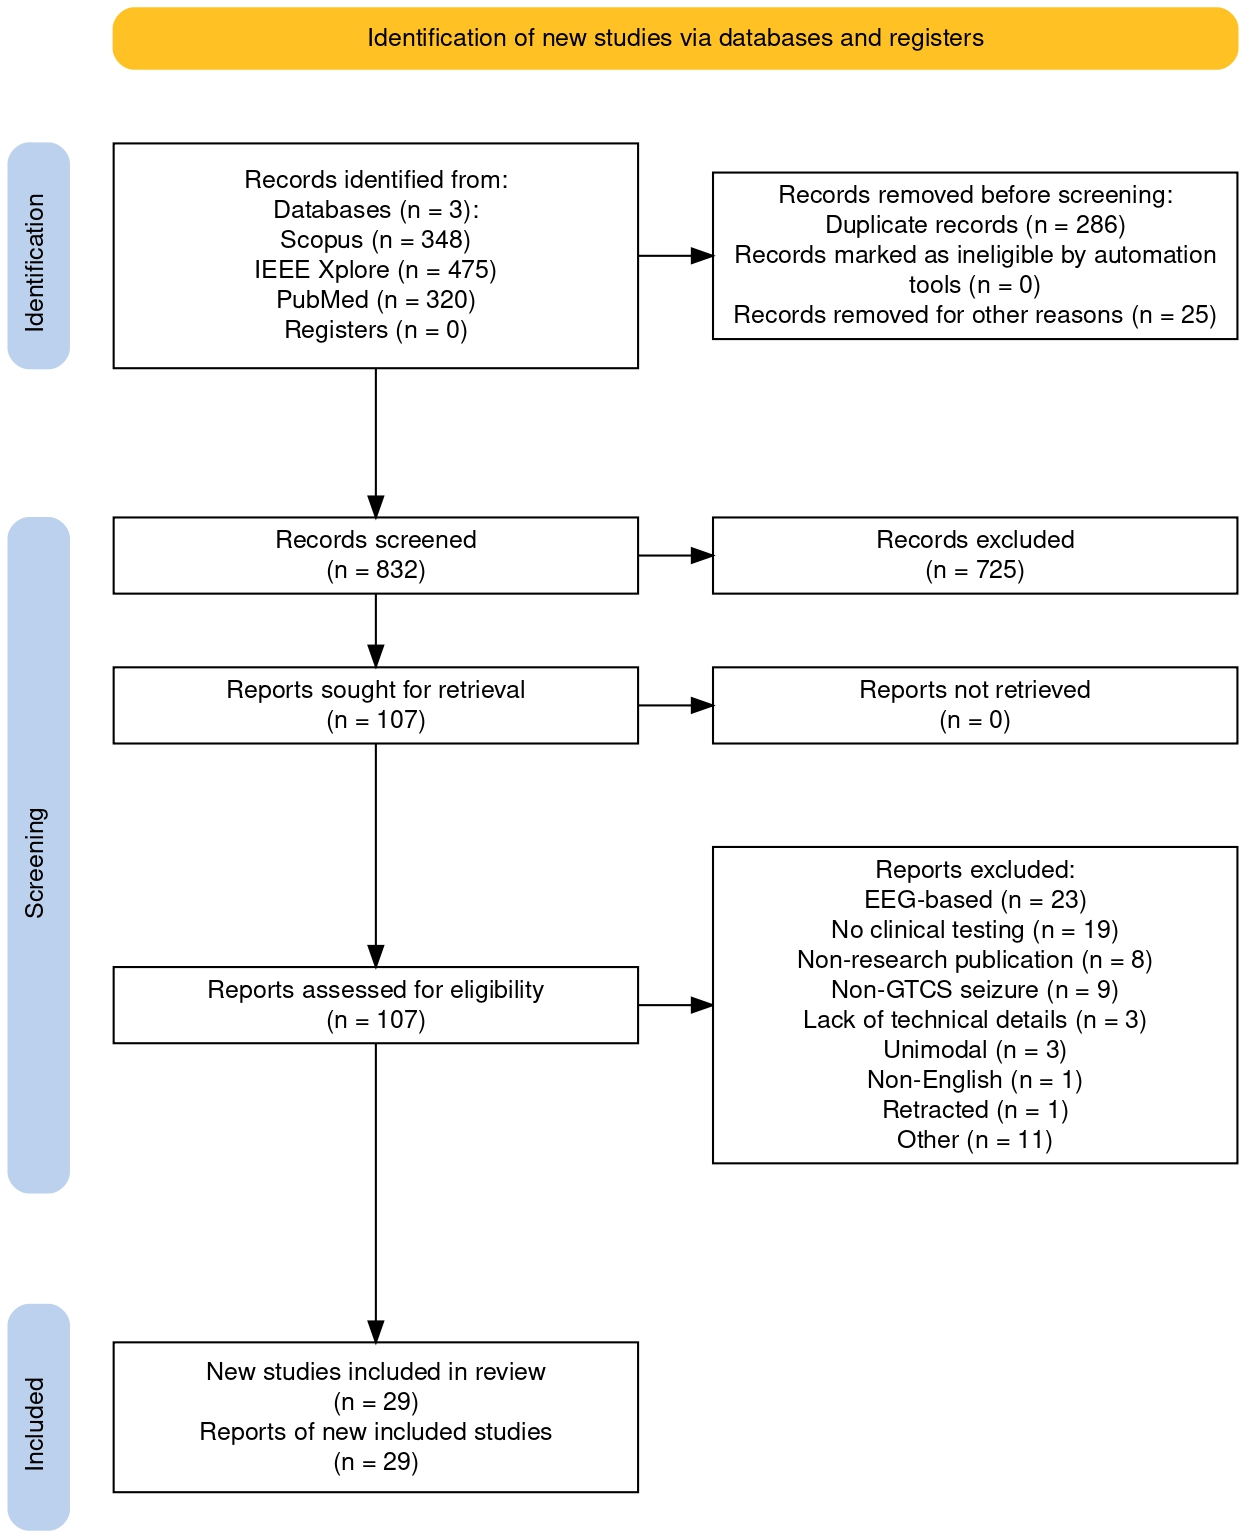
\includegraphics[width=1\textwidth]{methodology/figures/prisma_flow_diagram.jpg}
    \caption{PRISMA Flow Diagram}
    \label{fig:prisma_flow_diagram}
\end{figure}

This scoping review was conducted in accordance with the PRISMA Extension for Scoping Reviews (PRISMA-ScR) guidelines (Figure \ref{fig:prisma_flow_diagram}) \cite{Tricco2018-bb}.

Conference papers and peer-reviewed articles of various study designs were included if they investigated wearable multimodal approaches for the detection or prediction of epileptic seizures. Studies were excluded if they (1) were review articles, (2) employed a unimodal detection system, (3) lacked clinical validation, or (4) targeted focal seizures only.

Three electronic databases (Scopus, IEEE Xplore, and PubMed) were searched until April 22, 2025  using Boolean operators, wildcards, and keywords relevant to epilepsy as shown in (\href{https://docs.google.com/document/d/1FJTEZIhRoBhq3tmehHFUZllaM-GqR_4c1j9waukcQow/edit?tab=t.0}{supplementary file SI}). 

After duplicates removal, retrieved articles were screened first by titles and abstracts, followed by reading through the full-text. Eight reviewers independently participated as pairs in screening. Screening decisions and record management were handled using Mendeley for reference organization and Google Sheets for collaborative screening. 

Data charting was conducted in duplicate by independent reviewers using Google Sheets. Reviewers extracted data deemed relevant to the review objectives including: year of publication; task type (detection, prediction, or forecasting); study characteristics (clinical setting,  average patient age, dataset size, targeted seizure types, and reference standard); device characteristics (wearability, commercial device name if applicable, and sensor placement); signal characteristics (sensor modalities, extracted biomarkers, and preprocessing steps); algorithm characteristics (task type, real-time applicability, patient-specific versus generalized model, and best-performing algorithm); and reported outcomes (performance metrics and key findings). 

Extracted data were synthesized and presented using structured tables (\href{https://docs.google.com/spreadsheets/d/1FjxwkHFbNDM84nuqg513gR_0vIVql-evoT1EMiqSYZU/edit?pli=1&gid=1255223968#gid=1255223968}{Table S1}, \href{https://docs.google.com/spreadsheets/d/1FjxwkHFbNDM84nuqg513gR_0vIVql-evoT1EMiqSYZU/edit?pli=1&gid=97270185#gid=97270185}{Table S2}).
Discrepancies during screening and data charting were resolved through collaborative discussion.
